\documentclass{beamer}		
\usepackage{ragged2e}
\usepackage{tikz-cd}
\usepackage{eulervm}
\usepackage{mathtools}
\usepackage{amsmath,calligra,mathrsfs}
\usepackage{graphicx,wrapfig,lipsum}
\usepackage{subcaption}


\usepackage{tikz, xparse}
\usetikzlibrary{arrows}
\usepackage{amssymb}
\usepackage{amsmath}
\usepackage{amsthm}
\usepackage{array}
\usepackage{appendix}
\newcolumntype{P}[1]{>{\centering\arraybackslash}p{#1}}
\usepackage[absolute,overlay]{textpos}

\usepackage{algorithm}
\usepackage[noend]{algpseudocode}
\usepackage[ruled,linesnumbered]{algorithm2e}

\usepackage[T1]{fontenc}
\usepackage{subcaption}

\usepackage{mathtools}

\usepackage{wrapfig}

\usepackage{amsthm}
\theoremstyle{plain}
\newtheorem{mytheorem}{Theorem}[frame]
\newtheorem{mylemma}[mytheorem]{Lemma}
\newtheorem{myproposition}[mytheorem]{Proposition}
\newtheorem{mycorollary}[mytheorem]{Corollary}
\newtheorem{myconjecture}[mytheorem]{Conjecture}
%\theorembodyfont{\rmfamily}
\theoremstyle{definition}
\newtheorem{mydefinition}[mytheorem]{Definition}
\newtheorem{myexample}[mytheorem]{Example}
\newtheorem{myassumption}[mytheorem]{Assumption}
% %\theoremstyle{remark}
\newtheorem{mynotation}[mytheorem]{Notation}
\newtheorem{myremark}[mytheorem]{Remark}
\newenvironment{myproof}{\begin{proof}}{\end{proof}}
%\newtheorem*{myproof}{Proof}{\itshape}{\rmfamily}

\newcommand\nbd{\nobreakdash-\hspace{0pt}}
\NewDocumentCommand \bord{g g} {\IfNoValueTF{#2}{%
	\IfNoValueTF{#1}{\partial}{\partial_{#1}}}{\partial_{#1}^{#2}}}
\newcommand\eqdef{\coloneqq}

\newcommand\celto{\Rightarrow}
\newcommand\incl{\hookrightarrow}
\newcommand\dmn[1]{\mathrm{dim}(#1)}
\newcommand\cp[1]{\,{\scriptstyle\#}_{#1}\,}
\newcommand\incliso{\stackrel{\sim}{\hookrightarrow}}


\newcommand\code[1]{\texttt{#1}}
\newcommand\data[1]{\mathsf{#1}}
\newcommand\grade[2]{#2_{#1}}
\newcommand\size[1]{\left|{#1}\right|}

\newcommand\submol{\sqsubseteq}

\theoremstyle{ittheorem}
\newtheorem{thm}{Theorem}[section]
\newtheorem{prop}[thm]{Proposition}
\newcommand{\btVFill}{\vskip 0pt plus 1filll}

\newcommand\maxel[1]{\mathscr{M}\!\textit{ax}\,#1}
\newcommand\orderings[2]{\mathscr{O}\!\textit{rd}_{#1}{#2}}
\newcommand\layerings[2]{\mathscr{L}\!\textit{ay}_{#1}{#2}}
\newcommand\order[2]{#2^{(#1)}}
\newcommand\set[1]{\left\{ {#1} \right\}}
\newcommand\maxflow[2]{\mathscr{M}_{#1}{#2}}


% \usepackage{enumitem}
% \setlist[itemize]{noitemsep, nolistsep}

\setlength\parindent{0pt}

\usetheme{Madrid}		% Sets basic formatting.  Lots of options, google "beamer themes"

\usecolortheme{dolphin}	% Sets the colour scheme.  Lots of options, google "beamer color themes"

\setbeamertemplate{navigation symbols}{}	% Manually changes one piece of formatting.  See what the difference is by commenting this line out.

\date{18 June 2024}	% Insert the date of your presentation. \today gives an unsurprising automatic date.

\title[Critical Pairs for String Diagram Rewriting]{\vspace{1.5cm} Group 2 - Critical Pairs for String Diagram Rewriting}	% Insert your title.  Depending on the theme you choose above, a "short title" might be useful, as it will appear on the footer of each slide.

\author[Adjoint School Group 2]{Anna Matsui, Innocent Obi, Guillaume Sabbagh, Leo Torres,\\ Diana Kessler, Juan Meleiro, Koko Muroya} % Insert your name

\makeatletter
\setbeamertemplate{footline}{
  \leavevmode%
  \hbox{%
  \begin{beamercolorbox}[wd=.3\paperwidth,ht=2.25ex,dp=1ex,center]{author in head/foot}%
    \usebeamerfont{author in head/foot}\insertshortauthor\expandafter\ifblank\expandafter{\beamer@shortinstitute}{}{~~(\insertshortinstitute)}
  \end{beamercolorbox}%
  \begin{beamercolorbox}[wd=.4\paperwidth,ht=2.25ex,dp=1ex,center]{title in head/foot}%
    \usebeamerfont{title in head/foot}\insertshorttitle
  \end{beamercolorbox}%
  \begin{beamercolorbox}[wd=.3\paperwidth,ht=2.25ex,dp=1ex,right]{date in head/foot}%
    \usebeamerfont{date in head/foot}\insertshortdate{}\hspace*{2em}
    \insertframenumber{} / \inserttotalframenumber\hspace*{2ex} 
  \end{beamercolorbox}}%
  \vskip0pt%
}
\makeatother

\begin{document} 	% Let's begin
\maketitle

% \begin{frame}{Critical Pairs for String Diagram Rewriting}
    
% \end{frame}

\begin{frame}[allowframebreaks]{Motivation}
Why do we care about string diagrams for term rewriting?
\begin{figure}
    \centering
    
\includegraphics[scale=0.2]{images/conspiracy.jpeg}
    \caption{Their (monoidal) structure \textit{absorbs} conspiracies}
    \label{fig:enter-label}
\end{figure}
\framebreak
\begin{figure}
    \centering
    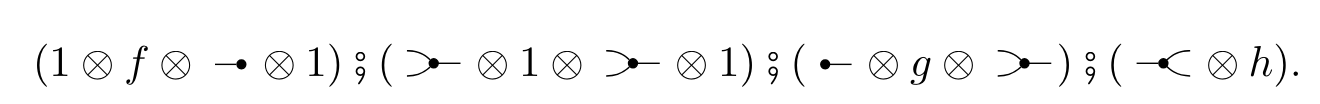
\includegraphics[scale=0.4]{images/string-diagram-example-one-d.png}
    \caption{1-dimensional(-ish) graphical syntax}
    \label{fig:enter-label}
\end{figure}
\begin{figure}
     \centering
 \begin{subfigure}[b]{0.3\textwidth}
         \centering
         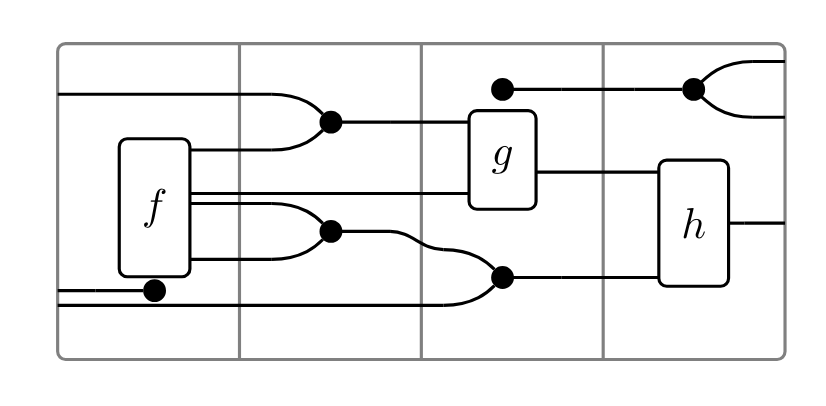
\includegraphics[width=\textwidth]{images/string-diagram-example.png}
         \caption{2-dimensional graphical syntax}
         \label{fig:three sin x}
     \end{subfigure}
     \hfill
     \begin{subfigure}[b]{0.3\textwidth}
         \centering
         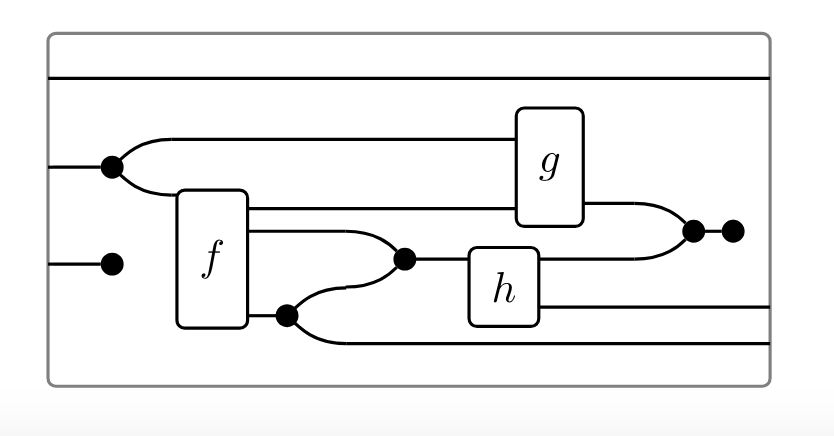
\includegraphics[width=\textwidth]{images/string-diagram-example-iso.png}
         \caption{2-dimensional graphical syntax}
         \label{fig:five over x}
     \end{subfigure}
    \hfill
     \begin{subfigure}[b]{0.3\textwidth}
         \centering
         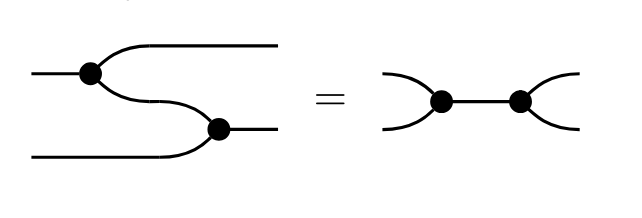
\includegraphics[width=\textwidth]{images/string-diagram-example-redex.png}
         \caption{equivalence modulo twisting and bending}
         \label{fig:five over x}
     \end{subfigure}
        \caption{Equivalences via 2-dimensional graphical syntax }
        \label{fig:three graphs}
\end{figure}
% \begin{figure}
%     \centering
%     \includegraphics{}
%     \caption{Caption}
%     \label{fig:enter-label}
% \end{figure}
%\begin{itemize}
%\justifying
%    \item With terms in an algebra, one-dimensional syntax can contain certain \textit{conspiracies} (equivalences or congruences) that are not obvious. 
%    \item Transformations on terms (rewrites) need to take into account this structure explicitly. Graphs transformations can do this implicitly.  
%    \item String diagrams are a two-dimensional (graphical) syntax for morphisms of monoidal categories which can be combinatorially presented as graphs.
%\framebreak
%    \item The symmetric monoidal category on a signature has as object lists of types from the signature and as morphisms equivalence class of well-typed terms. 
%    \item Two-dimensional syntax can represent congruence naturally (terms quotiented by equivalences) as isomorphic graphs 
%    \item But there is a negative result to contend with: \textbf{undeciability of confluence}.
%\end{itemize}
\end{frame}

\begin{frame}[allowframebreaks]{Confluence of rewriting systems}
\begin{myexample}[From \cite{DBLP:journals/mscs/BonchiGKSZ22a}]
    Given the signature $\Sigma = \{ \gamma : 2 \rightarrow 2 \}$ and the rewriting system $S_{\Sigma}$: 
\begin{figure}
    \centering
    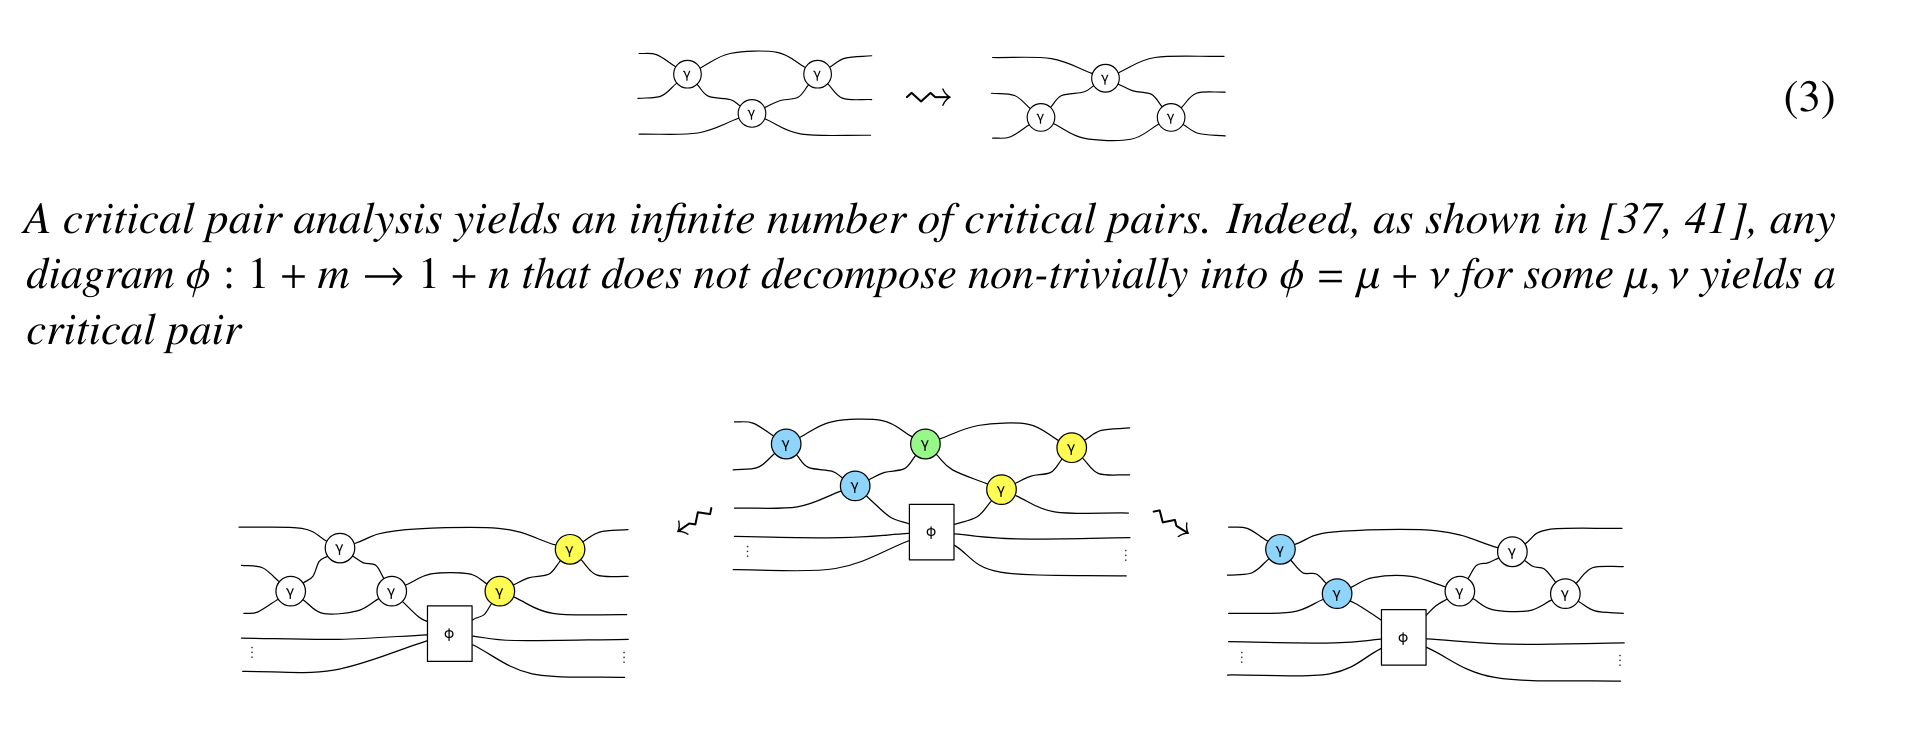
\includegraphics[scale=0.3]{images/cp-example.png}
    \caption{Redex overlap resulting in separate embeddings.  }
    \label{fig:enter-label}
\end{figure}
\end{myexample}

\framebreak
\begin{mytheorem}[Decidability of Confluence \cite{Plump1994CriticalPI}]
    A finite, terminating term rewriting system is confluent if and only if all critical pairs are (strongly) joinable. \footnote{this is equivalent to the Knuth-Bendix property for string and term rewriting systems}
\end{mytheorem}
\begin{mytheorem}[Undecidability of Confluence \cite{Plump1993HypergraphRC}]
It is undecidable in general whether a finite, terminating hypergraph rewriting system is confluent
\end{mytheorem}
\begin{figure}
    \centering
    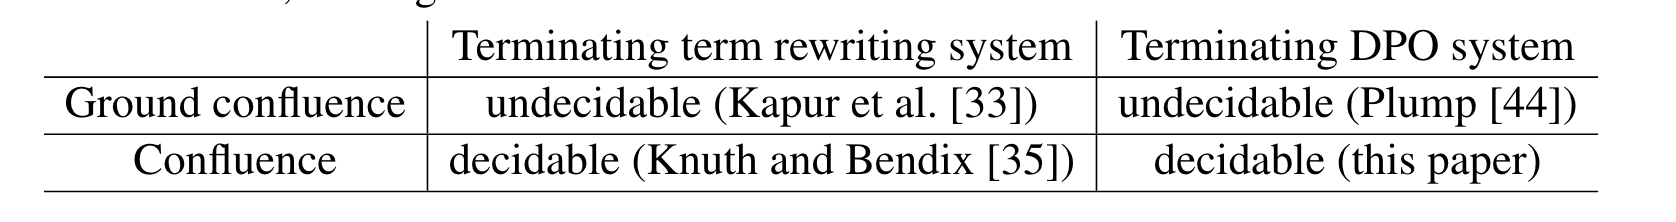
\includegraphics[scale=0.4]{images/confluence_table.png}
    \caption{Decidability of Confluence for Rewriting Systems \cite{DBLP:journals/mscs/BonchiGKSZ22a}}
    \label{fig:enter-label}
\end{figure}

%Joinability of critical pairs \textbf{does not entail} confluence.
%\item Confluence --- "Do two different rewrites converge?"

\framebreak
\[\begin{tikzcd}[ampersand replacement=\&, column sep=small]
	L \& K \& R \&\& L \& K \& R \\
	G \& C \& H \&\& G \& C \& H \\
	\&\&\&\&\& J
	\arrow[from=1-1, to=2-1]
	\arrow[from=1-2, to=1-1]
	\arrow[from=1-2, to=1-3]
	\arrow[from=1-2, to=2-2]
	\arrow[""{name=0, anchor=center, inner sep=0}, from=1-3, to=2-3]
	\arrow[""{name=1, anchor=center, inner sep=0}, from=1-5, to=2-5]
	\arrow[from=1-6, to=1-5]
	\arrow[from=1-6, to=1-7]
	\arrow[from=1-6, to=2-6]
	\arrow[from=1-7, to=2-7]
	\arrow["\lrcorner"{anchor=center, pos=0.125, rotate=90}, draw=none, from=2-1, to=1-2]
	\arrow[from=2-2, to=2-1]
	\arrow[from=2-2, to=2-3]
	\arrow["\lrcorner"{anchor=center, pos=0.125, rotate=180}, draw=none, from=2-3, to=1-2]
	\arrow["\lrcorner"{anchor=center, pos=0.125, rotate=90}, draw=none, from=2-5, to=1-6]
	\arrow[from=2-6, to=2-5]
	\arrow[from=2-6, to=2-7]
	\arrow["\lrcorner"{anchor=center, pos=0.125, rotate=180}, draw=none, from=2-7, to=1-6]
	\arrow[from=3-6, to=2-5]
	\arrow[from=3-6, to=2-6]
	\arrow[from=3-6, to=2-7]
	\arrow[shorten <=19pt, shorten >=19pt, Rightarrow, from=0, to=1]
\end{tikzcd}
\]
\begin{itemize}
\justifying
    \item \cite{DBLP:journals/mscs/BonchiGKSZ22a}: String diagram rewriting, formalized using double pushout (DPO) with interfaces, preserves the Knuth-Bendix property: \textit{Confluence of a terminating DPOI system can be decided by checking whether its critical pairs are joinable.}
    %\item (Interfaces)String diagrams have a natural notion of interfaces: inputs and outputs of diagram represent domain and codomain of a morphism in a symmetric monoidal category.
    %\item (Interfaces give up. We do this in SMC with Frobenius strucutre)
    %\item (left-linearity for monogamrous graphs)
    %\item so we wget...
    %\item Despite the negative result in Plump, we know that with an SMC with a Frobenius structure (and in generic adhesive categories), confluence of DPO with interfaces (DPOI) is decidable. And this can be done by checking joinability of critical pairs. 
    \item Confluence of DPOI rewriting system $\Rightarrow$ Confluence of $ \mathbf{S}_{\Sigma} + \mathbf{Frob}$
\end{itemize}
% \pause 6669aae01e91262e373347e5

\end{frame}
\begin{frame}{Goal(s) for Research Week}
\begin{enumerate}
    \item \textbf{Enumerating critical pairs.} Building on efforts in the automation of confluence proofs (CoCo completion project). How can we enumerate all critical pairs for a given DPOI rewriting system?
\end{enumerate}
\end{frame}
%  String diagram rewriting: modeling dynamics of systems

\begin{frame}{Basic definitions - \cite{DBLP:journals/mscs/BonchiGKSZ22a}}
\begin{itemize}
\justifying
%https://q.uiver.app/#q=WzAsNyxbMCwwLCJMIl0sWzEsMCwiSyJdLFsyLDAsIlIiXSxbMiwxLCJIIl0sWzAsMSwiRyJdLFsxLDEsIkMiXSxbMSwyLCJKIl0sWzEsMF0sWzEsMl0sWzEsNV0sWzIsM10sWzAsNCwibSIsMl0sWzUsNF0sWzUsM10sWzYsNV0sWzYsM10sWzYsNF0sWzQsMSwiIiwyLHsic3R5bGUiOnsibmFtZSI6ImNvcm5lciJ9fV0sWzMsMSwiIiwyLHsic3R5bGUiOnsibmFtZSI6ImNvcm5lciJ9fV1d
\item The double pushout with interfaces rewrite rule: We say $(G \to J)\rightsquigarrow (H \to J) $ if there exists a rewrite rule $L \leftarrow K \to R$ and an object $C$ with suitable morphisms such that the diagram below commutes and the squares are pushouts
\[\begin{tikzcd}[ampersand replacement=\&, column sep=small]
	L \& K \& R \\
	G \& C \& H \\
	\& J
	\arrow["m", from=1-1, to=2-1]
	\arrow[from=1-2, to=1-1]
	\arrow[from=1-2, to=1-3]
	\arrow[from=1-2, to=2-2]
	\arrow[from=1-3, to=2-3]
	\arrow["\lrcorner"{anchor=center, pos=0.125, rotate=90}, draw=none, from=2-1, to=1-2]
	\arrow[from=2-2, to=2-1]
	\arrow[from=2-2, to=2-3]
	\arrow["\lrcorner"{anchor=center, pos=0.125, rotate=180}, draw=none, from=2-3, to=1-2]
	\arrow[from=3-2, to=2-1]
	\arrow[from=3-2, to=2-2]
	\arrow[from=3-2, to=2-3]
\end{tikzcd}\]
\end{itemize}
\end{frame}

\begin{frame}{Example - \cite{Bonchi2020StringDR}}
    \centering
    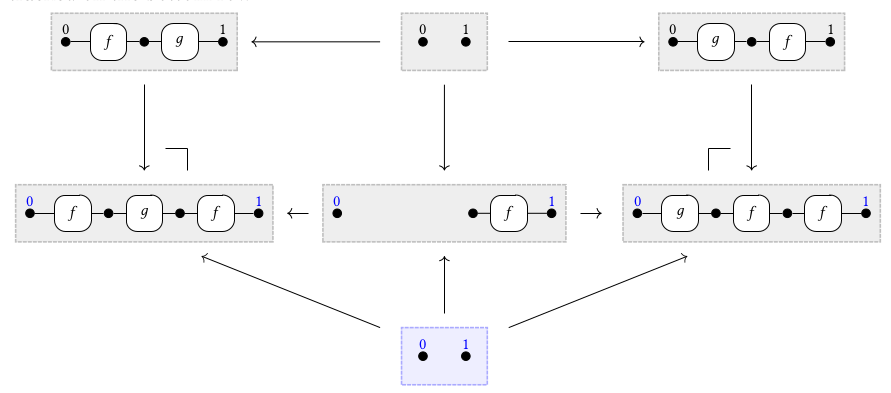
\includegraphics[scale = 0.32]{images/DP_rewrite.png}
\end{frame}

\begin{frame}{Basic definitions - \cite{DBLP:journals/mscs/BonchiGKSZ22a} }
\begin{itemize}
    \item Pre-critical pair: We say $(H_1 \leftarrow J) \rightsquigarrow (S \leftarrow J)  \rightsquigarrow  (H_2 \leftarrow J)$ is a precritical pair if in the following diagram $[f_1,f_2]:L_1+L_2 \to S$ is epi and * is a pullback
    
    % morphismshttps://q.uiver.app/#q=WzAsMTIsWzAsMCwiUl8xIl0sWzEsMCwiS18xIl0sWzIsMCwiTF8xIl0sWzQsMCwiTF8yIl0sWzUsMCwiS18yIl0sWzMsMSwiUyJdLFswLDEsIkhfMSJdLFsxLDEsIkNfMSJdLFs1LDEsIkNfMiJdLFs2LDEsIkhfMiJdLFs2LDAsIlJfMiJdLFszLDIsIkoiXSxbMSwyXSxbMSwwXSxbNCwzXSxbNCwxMF0sWzMsNSwiZl8yIiwyXSxbMiw1LCJmXzEiXSxbNyw2XSxbMCw2XSxbMSw3XSxbOCw1XSxbOCw5XSxbMTAsOV0sWzQsOF0sWzYsMSwiIiwxLHsic3R5bGUiOnsibmFtZSI6ImNvcm5lciJ9fV0sWzUsMSwiIiwxLHsic3R5bGUiOnsibmFtZSI6ImNvcm5lciJ9fV0sWzUsNCwiIiwxLHsic3R5bGUiOnsibmFtZSI6ImNvcm5lciJ9fV0sWzExLDhdLFsxMSw3XSxbMTEsNSwiKiIsMSx7ImxhYmVsX3Bvc2l0aW9uIjowLCJzdHlsZSI6eyJib2R5Ijp7Im5hbWUiOiJub25lIn19fV0sWzcsNSwiIiwyLHsibGFiZWxfcG9zaXRpb24iOjQwfV0sWzksNCwiIiwyLHsic3R5bGUiOnsibmFtZSI6ImNvcm5lciJ9fV1d
\[\begin{tikzcd}[ampersand replacement=\&, column sep=small]
	{R_1} \& {K_1} \& {L_1} \&\& {L_2} \& {K_2} \& {R_2} \\
	{H_1} \& {C_1} \&\& S \&\& {C_2} \& {H_2} \\
	\&\&\& {\overset{*}{J}}
	\arrow[from=1-1, to=2-1]
	\arrow[from=1-2, to=1-1]
	\arrow[from=1-2, to=1-3]
	\arrow[from=1-2, to=2-2]
	\arrow["{f_1}", from=1-3, to=2-4]
	\arrow["{f_2}"', from=1-5, to=2-4]
	\arrow[from=1-6, to=1-5]
	\arrow[from=1-6, to=1-7]
	\arrow[from=1-6, to=2-6]
	\arrow[from=1-7, to=2-7]
	\arrow["\lrcorner"{anchor=center, pos=0.125, rotate=90}, draw=none, from=2-1, to=1-2]
	\arrow[from=2-2, to=2-1]
	\arrow[from=2-2, to=2-4]
	\arrow["\lrcorner"{anchor=center, pos=0.125, rotate=180}, draw=none, from=2-4, to=1-2]
	\arrow["\lrcorner"{anchor=center, pos=0.125, rotate=90}, draw=none, from=2-4, to=1-6]
	\arrow[from=2-6, to=2-4]
	\arrow[from=2-6, to=2-7]
	\arrow["\lrcorner"{anchor=center, pos=0.125, rotate=180}, draw=none, from=2-7, to=1-6]
	\arrow[from=3-4, to=2-2]
	\arrow[from=3-4, to=2-6]
\end{tikzcd}\]
\end{itemize}
\end{frame}

\begin{frame}{Basic definitions - \cite{DBLP:journals/mscs/BonchiGKSZ22a} }
\begin{itemize}
\item Parallel pair

In the setting of the previous definition, we say that the pre-critical pair is parallel if there exist morphisms $L_1 \rightarrow C_2$ and $L_2 \rightarrow C_1$ making the diagram below commute  
% https://q.uiver.app/#q=WzAsNyxbMCwwLCJLXzEiXSxbMSwwLCJMXzEiXSxbMywwLCJMXzIiXSxbNCwwLCJLXzIiXSxbMCwxLCJDXzEiXSxbMiwxLCJTIl0sWzQsMSwiQ18yIl0sWzAsMSwiZl8xIiwwLHsic3R5bGUiOnsidGFpbCI6eyJuYW1lIjoiaG9vayIsInNpZGUiOiJ0b3AifX19XSxbMCw0XSxbMSw1XSxbMSw2XSxbMiw1XSxbMiw0XSxbMywyLCJmXzIiLDIseyJzdHlsZSI6eyJ0YWlsIjp7Im5hbWUiOiJob29rIiwic2lkZSI6InRvcCJ9fX1dLFszLDZdLFs0LDVdLFs2LDVdXQ==
\[\begin{tikzcd}[ampersand replacement=\&, column sep=small]
	{K_1} \& {L_1} \&\& {L_2} \& {K_2} \\
	{C_1} \&\& S \&\& {C_2}
	\arrow["{f_1}", hook, from=1-1, to=1-2]
	\arrow[from=1-1, to=2-1]
	\arrow[from=1-2, to=2-3]
	\arrow[from=1-2, to=2-5]
	\arrow[from=1-4, to=2-1]
	\arrow[from=1-4, to=2-3]
	\arrow["{f_2}"', hook, from=1-5, to=1-4]
	\arrow[from=1-5, to=2-5]
	\arrow[from=2-1, to=2-3]
        \arrow[from=2-5, to=2-3]
\end{tikzcd}\]
Note: the key result and reason for distinction is that parallel pairs are always joinable.
\end{itemize}
\end{frame}

\begin{frame}{Basic definitions - \cite{DBLP:journals/mscs/BonchiGKSZ22a} }
\begin{itemize}
    \item Parallel pair (with interface)

In the setting pf pre-critical pairs, consider the diagram below formed by pullbacks. We say that the pair is parallel, $X \rightarrow L_1$ and $Y \rightarrow L_2$ are iso and $C_1 \rightarrow S$ and $C_2 \rightarrow S$ are mono.
% https://q.uiver.app/#q=WzAsOCxbMSwwLCJMXzEiXSxbMywwLCJMXzIiXSxbMCwxLCJYIl0sWzIsMSwiUyJdLFs0LDEsIlkiXSxbMSwyLCJDXzIiXSxbMywyLCJDXzEiXSxbMiwzLCJKIl0sWzAsM10sWzEsM10sWzIsNV0sWzIsMF0sWzQsMV0sWzQsNl0sWzUsM10sWzYsM10sWzcsNV0sWzcsNl1d
\[\begin{tikzcd}[ampersand replacement=\&, column sep=small]
	\& {L_1} \&\& {L_2} \\
	X \&\& S \&\& Y \\
	\& {C_2} \&\& {C_1} \\
	\&\& J
	\arrow[from=1-2, to=2-3]
	\arrow[from=1-4, to=2-3]
	\arrow[from=2-1, to=1-2]
	\arrow[from=2-1, to=3-2]
	\arrow[from=2-5, to=1-4]
	\arrow[from=2-5, to=3-4]
	\arrow[from=3-2, to=2-3]
	\arrow[from=3-4, to=2-3]
	\arrow[from=4-3, to=3-2]
	\arrow[from=4-3, to=3-4]
\end{tikzcd}\]
\footnote{Note: for the rewrite systems that we are considering (left-linear), the definition coincides with that without interfaces (assume $X = L_1$ and $Y = L_2$)}
\end{itemize}
\end{frame}

% \begin{frame}[allowframebreaks]{Basic definitions - \cite{DBLP:journals/mscs/BonchiGKSZ22a}}

% \begin{itemize}
% \justifying
% %https://q.uiver.app/#q=WzAsNyxbMCwwLCJMIl0sWzEsMCwiSyJdLFsyLDAsIlIiXSxbMiwxLCJIIl0sWzAsMSwiRyJdLFsxLDEsIkMiXSxbMSwyLCJKIl0sWzEsMF0sWzEsMl0sWzEsNV0sWzIsM10sWzAsNCwibSIsMl0sWzUsNF0sWzUsM10sWzYsNV0sWzYsM10sWzYsNF0sWzQsMSwiIiwyLHsic3R5bGUiOnsibmFtZSI6ImNvcm5lciJ9fV0sWzMsMSwiIiwyLHsic3R5bGUiOnsibmFtZSI6ImNvcm5lciJ9fV1d
% \item The double pushout with interfaces rewrite rule: We say $(G \to J)\rightsquigarrow (H \to J) $ if there exists a rewrite rule $L \leftarrow K \to R$ and an object $C$ with suitable morphisms such that the diagram below commutes and the squares are pushouts
% \[\begin{tikzcd}[ampersand replacement=\&, column sep=small]
% 	L \& K \& R \\
% 	G \& C \& H \\
% 	\& J
% 	\arrow["m", from=1-1, to=2-1]
% 	\arrow[from=1-2, to=1-1]
% 	\arrow[from=1-2, to=1-3]
% 	\arrow[from=1-2, to=2-2]
% 	\arrow[from=1-3, to=2-3]
% 	\arrow["\lrcorner"{anchor=center, pos=0.125, rotate=90}, draw=none, from=2-1, to=1-2]
% 	\arrow[from=2-2, to=2-1]
% 	\arrow[from=2-2, to=2-3]
% 	\arrow["\lrcorner"{anchor=center, pos=0.125, rotate=180}, draw=none, from=2-3, to=1-2]
% 	\arrow[from=3-2, to=2-1]
% 	\arrow[from=3-2, to=2-2]
% 	\arrow[from=3-2, to=2-3]
% \end{tikzcd}\]

% %\break

% %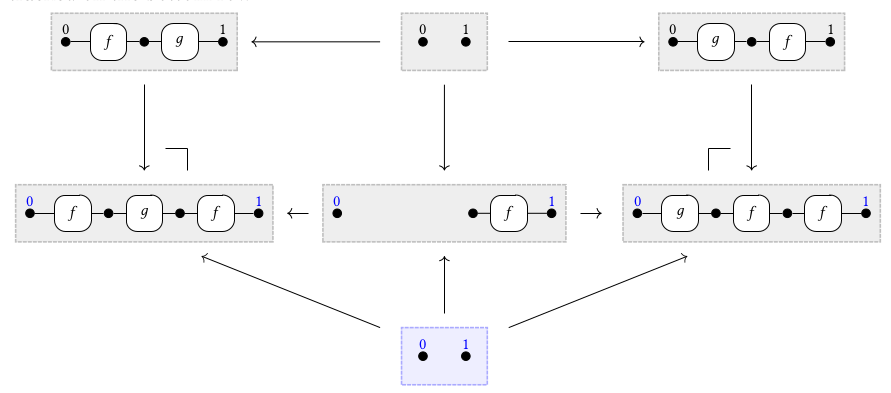
\includegraphics[scale = 0.26]{images/DP_rewrite.png}

% \framebreak
% \item Pre-critical pair: We say $(H_1 \leftarrow J) \rightsquigarrow (S \leftarrow J)  \rightsquigarrow  (H_2 \leftarrow J)$ is a precritical pair if in the following diagram $[f_1,f_2]:L_1+L_2 \to S$ is epi and * is a pullback
    
%     % morphismshttps://q.uiver.app/#q=WzAsMTIsWzAsMCwiUl8xIl0sWzEsMCwiS18xIl0sWzIsMCwiTF8xIl0sWzQsMCwiTF8yIl0sWzUsMCwiS18yIl0sWzMsMSwiUyJdLFswLDEsIkhfMSJdLFsxLDEsIkNfMSJdLFs1LDEsIkNfMiJdLFs2LDEsIkhfMiJdLFs2LDAsIlJfMiJdLFszLDIsIkoiXSxbMSwyXSxbMSwwXSxbNCwzXSxbNCwxMF0sWzMsNSwiZl8yIiwyXSxbMiw1LCJmXzEiXSxbNyw2XSxbMCw2XSxbMSw3XSxbOCw1XSxbOCw5XSxbMTAsOV0sWzQsOF0sWzYsMSwiIiwxLHsic3R5bGUiOnsibmFtZSI6ImNvcm5lciJ9fV0sWzUsMSwiIiwxLHsic3R5bGUiOnsibmFtZSI6ImNvcm5lciJ9fV0sWzUsNCwiIiwxLHsic3R5bGUiOnsibmFtZSI6ImNvcm5lciJ9fV0sWzExLDhdLFsxMSw3XSxbMTEsNSwiKiIsMSx7ImxhYmVsX3Bvc2l0aW9uIjowLCJzdHlsZSI6eyJib2R5Ijp7Im5hbWUiOiJub25lIn19fV0sWzcsNSwiIiwyLHsibGFiZWxfcG9zaXRpb24iOjQwfV0sWzksNCwiIiwyLHsic3R5bGUiOnsibmFtZSI6ImNvcm5lciJ9fV1d
% \[\begin{tikzcd}[ampersand replacement=\&, column sep=small]
% 	{R_1} \& {K_1} \& {L_1} \&\& {L_2} \& {K_2} \& {R_2} \\
% 	{H_1} \& {C_1} \&\& S \&\& {C_2} \& {H_2} \\
% 	\&\&\& {\overset{*}{J}}
% 	\arrow[from=1-1, to=2-1]
% 	\arrow[from=1-2, to=1-1]
% 	\arrow[from=1-2, to=1-3]
% 	\arrow[from=1-2, to=2-2]
% 	\arrow["{f_1}", from=1-3, to=2-4]
% 	\arrow["{f_2}"', from=1-5, to=2-4]
% 	\arrow[from=1-6, to=1-5]
% 	\arrow[from=1-6, to=1-7]
% 	\arrow[from=1-6, to=2-6]
% 	\arrow[from=1-7, to=2-7]
% 	\arrow["\lrcorner"{anchor=center, pos=0.125, rotate=90}, draw=none, from=2-1, to=1-2]
% 	\arrow[from=2-2, to=2-1]
% 	\arrow[from=2-2, to=2-4]
% 	\arrow["\lrcorner"{anchor=center, pos=0.125, rotate=180}, draw=none, from=2-4, to=1-2]
% 	\arrow["\lrcorner"{anchor=center, pos=0.125, rotate=90}, draw=none, from=2-4, to=1-6]
% 	\arrow[from=2-6, to=2-4]
% 	\arrow[from=2-6, to=2-7]
% 	\arrow["\lrcorner"{anchor=center, pos=0.125, rotate=180}, draw=none, from=2-7, to=1-6]
% 	\arrow[from=3-4, to=2-2]
% 	\arrow[from=3-4, to=2-6]
% \end{tikzcd}\]



% \framebreak

% \item Parallel pair

% In the setting of the previous definition, we say that the pre-critical pair is parallel if there exist morphisms $L_1 \rightarrow C_2$ and $L_2 \rightarrow C_1$ making the diagram below commute  
% % https://q.uiver.app/#q=WzAsNyxbMCwwLCJLXzEiXSxbMSwwLCJMXzEiXSxbMywwLCJMXzIiXSxbNCwwLCJLXzIiXSxbMCwxLCJDXzEiXSxbMiwxLCJTIl0sWzQsMSwiQ18yIl0sWzAsMSwiZl8xIiwwLHsic3R5bGUiOnsidGFpbCI6eyJuYW1lIjoiaG9vayIsInNpZGUiOiJ0b3AifX19XSxbMCw0XSxbMSw1XSxbMSw2XSxbMiw1XSxbMiw0XSxbMywyLCJmXzIiLDIseyJzdHlsZSI6eyJ0YWlsIjp7Im5hbWUiOiJob29rIiwic2lkZSI6InRvcCJ9fX1dLFszLDZdLFs0LDVdLFs2LDVdXQ==
% \[\begin{tikzcd}[ampersand replacement=\&, column sep=small]
% 	{K_1} \& {L_1} \&\& {L_2} \& {K_2} \\
% 	{C_1} \&\& S \&\& {C_2}
% 	\arrow["{f_1}", hook, from=1-1, to=1-2]
% 	\arrow[from=1-1, to=2-1]
% 	\arrow[from=1-2, to=2-3]
% 	\arrow[from=1-2, to=2-5]
% 	\arrow[from=1-4, to=2-1]
% 	\arrow[from=1-4, to=2-3]
% 	\arrow["{f_2}"', hook, from=1-5, to=1-4]
% 	\arrow[from=1-5, to=2-5]
% 	\arrow[from=2-1, to=2-3]
%         \arrow[from=2-5, to=2-3]
% \end{tikzcd}\]
% Note: the key result and reason for distinction is that parallel pairs are always joinable.

% \framebreak

% \item Parallel pair (with interface)

% In the setting pf pre-critical pairs, consider the diagram below formed by pullbacks. We say that the pair is parallel, $X \rightarrow L_1$ and $Y \rightarrow L_2$ are iso and $C_1 \rightarrow S$ and $C_2 \rightarrow S$ are mono.
% % https://q.uiver.app/#q=WzAsOCxbMSwwLCJMXzEiXSxbMywwLCJMXzIiXSxbMCwxLCJYIl0sWzIsMSwiUyJdLFs0LDEsIlkiXSxbMSwyLCJDXzIiXSxbMywyLCJDXzEiXSxbMiwzLCJKIl0sWzAsM10sWzEsM10sWzIsNV0sWzIsMF0sWzQsMV0sWzQsNl0sWzUsM10sWzYsM10sWzcsNV0sWzcsNl1d
% \[\begin{tikzcd}[ampersand replacement=\&, column sep=small]
% 	\& {L_1} \&\& {L_2} \\
% 	X \&\& S \&\& Y \\
% 	\& {C_2} \&\& {C_1} \\
% 	\&\& J
% 	\arrow[from=1-2, to=2-3]
% 	\arrow[from=1-4, to=2-3]
% 	\arrow[from=2-1, to=1-2]
% 	\arrow[from=2-1, to=3-2]
% 	\arrow[from=2-5, to=1-4]
% 	\arrow[from=2-5, to=3-4]
% 	\arrow[from=3-2, to=2-3]
% 	\arrow[from=3-4, to=2-3]
% 	\arrow[from=4-3, to=3-2]
% 	\arrow[from=4-3, to=3-4]
% \end{tikzcd}\]
% \footnote{Note: for the rewrite systems that we are considering (left-linear), the definition coincides with that without interfaces (assume $X = L_1$ and $Y = L_2$)}
% \end{itemize}
% \end{frame}


\begin{frame}{Example 1 - \cite{DBLP:journals/mscs/BonchiGKSZ22a}}
    \vspace{-0.5cm}
   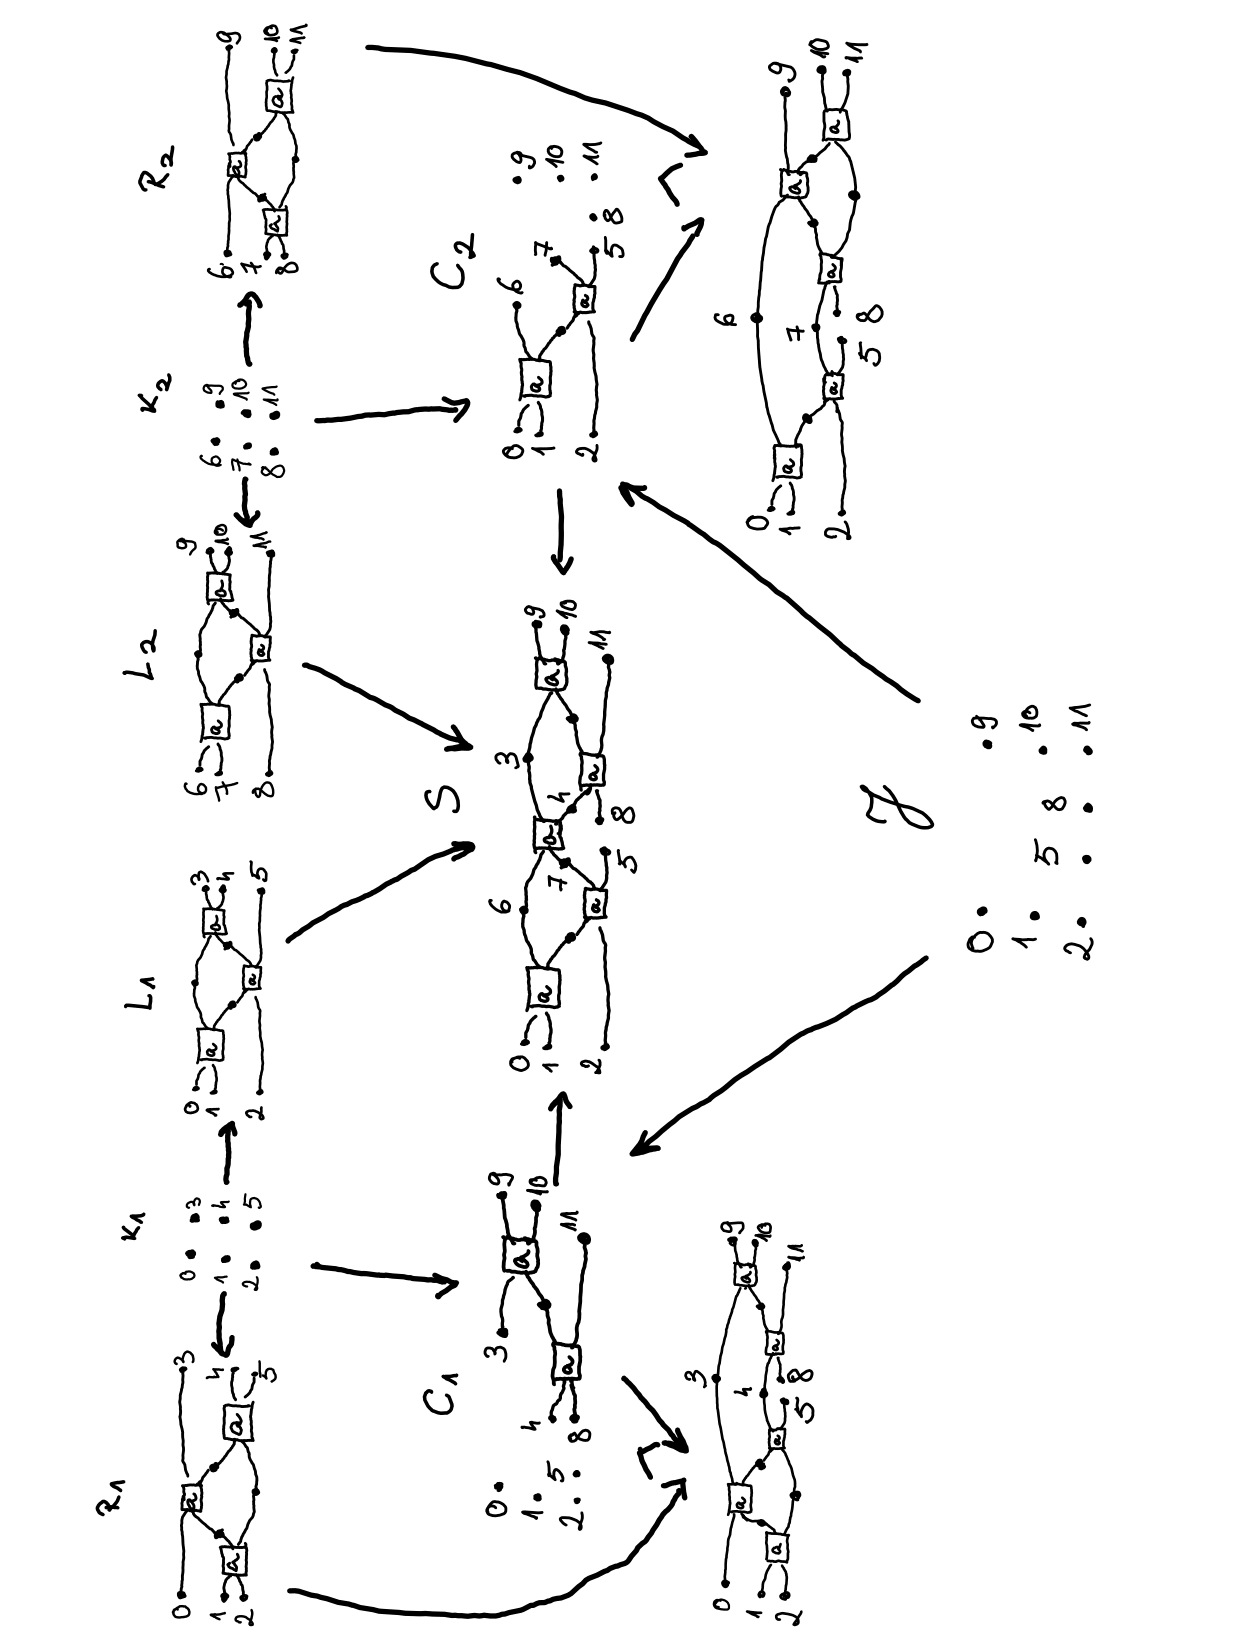
\includegraphics[scale=0.57 ,angle=270]{images/cp_example.png} 
\end{frame}

\begin{frame}{Example 2 - parallel pair}
    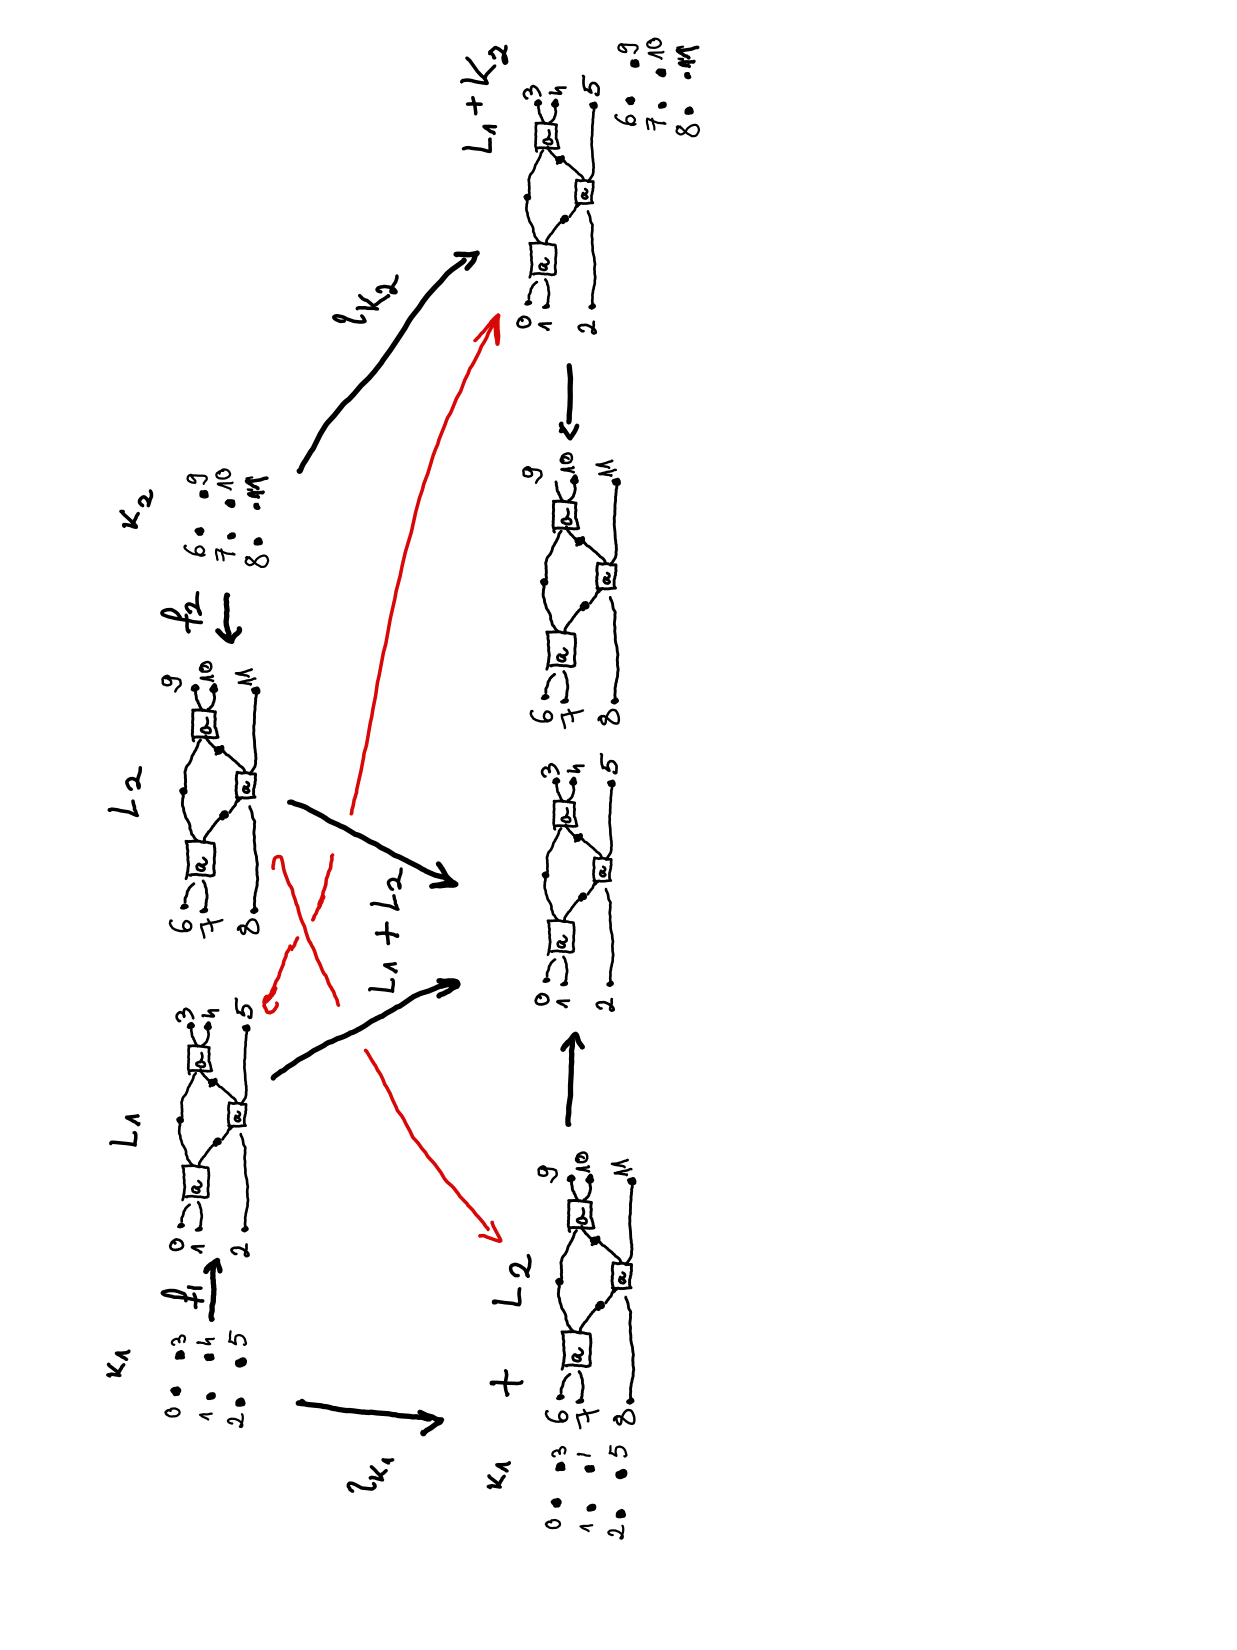
\includegraphics[scale = 0.58,angle=270]{images/cp_parallel.png}
\end{frame}

% \begin{frame}{The Algorithm}
%    \hspace{1.75cm}
%    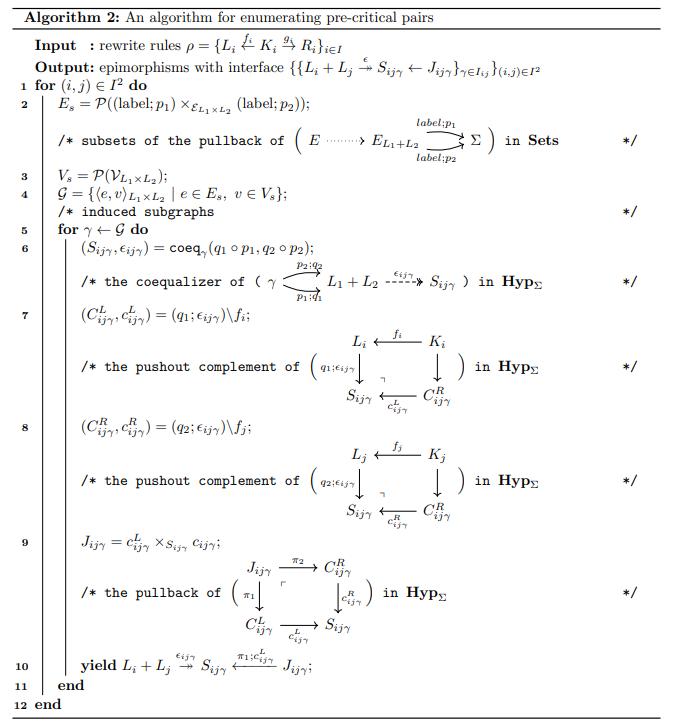
\includegraphics[scale=0.4]{images/algorithm.png} 


% \end{frame}

\begin{frame}[allowframebreaks]{The Algorithm - example}
Consider two rewrite rules:
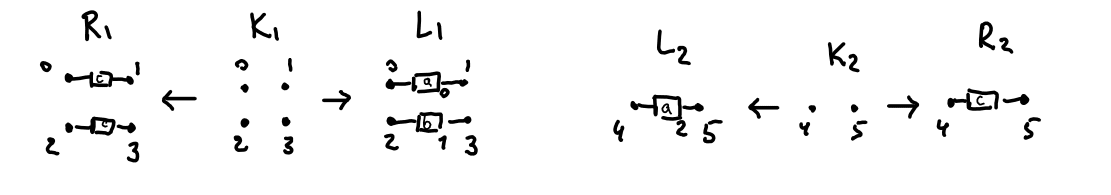
\includegraphics[scale=0.5]{images/2rewrites.png}
%\pause
First, compute the hypergraph $L_1 \times L_2$:% + V(L_1)^2 + V(L_2)^2$:
\begin{center}
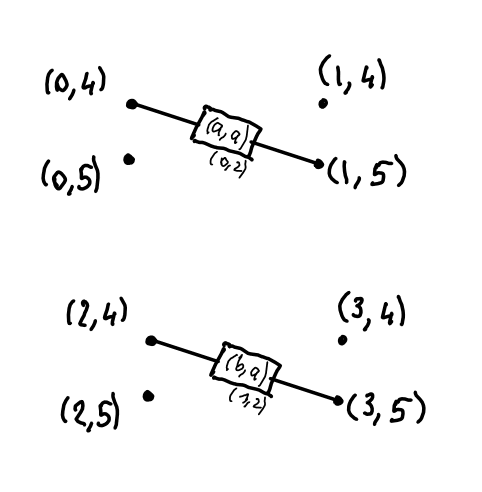
\includegraphics[scale=0.4]{images/l1l2.png}
\end{center}
%\pause
Now, we leave only the compatible pairs:
\begin{center}
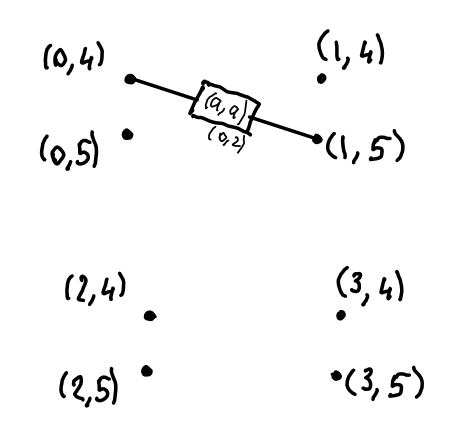
\includegraphics[scale=0.4]{images/compatible.png}
\end{center}
\framebreak

For every subgraph, compute the glueing. 

For example, for glueing 
\begin{center}
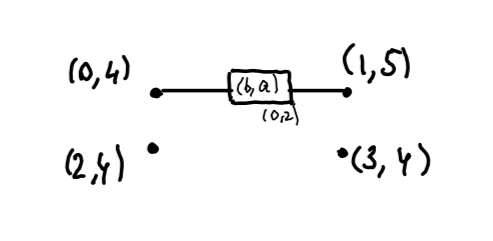
\includegraphics[scale=0.5]{images/tbglued.png}
\end{center}
%\pause
we get 
\begin{center}
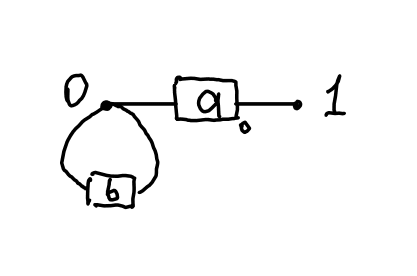
\includegraphics[scale=0.5]{images/res.png}
\end{center}

Also check the necessary conditions (ma-hypergraph, glueing condition for pushout complements).

\framebreak

Compute the pushout complements and the interface, and yield
\begin{center}
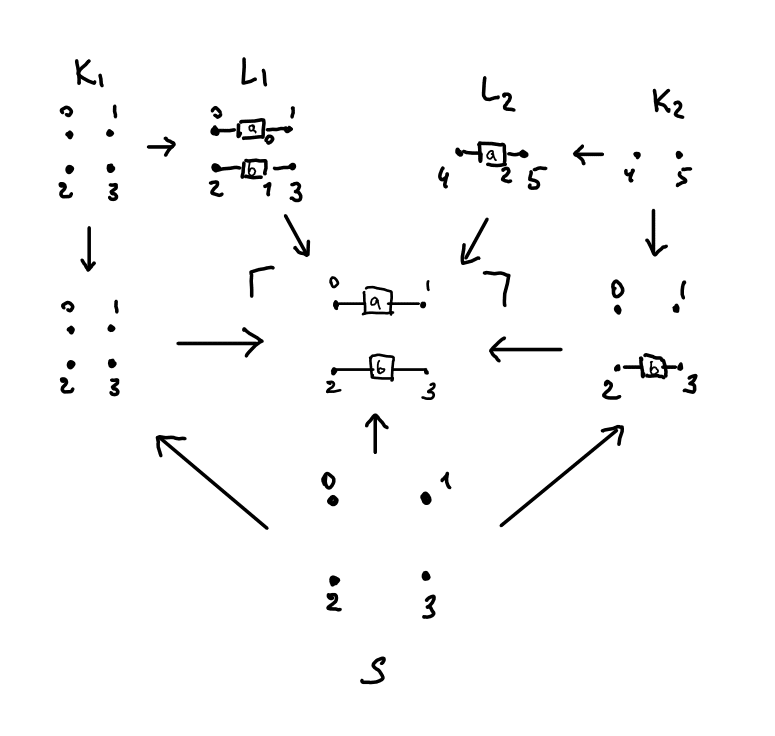
\includegraphics[scale=0.7]{images/crit.png}
\end{center}
\end{frame}

\begin{frame}{The Algorithm}
   \hspace{1.75cm}
   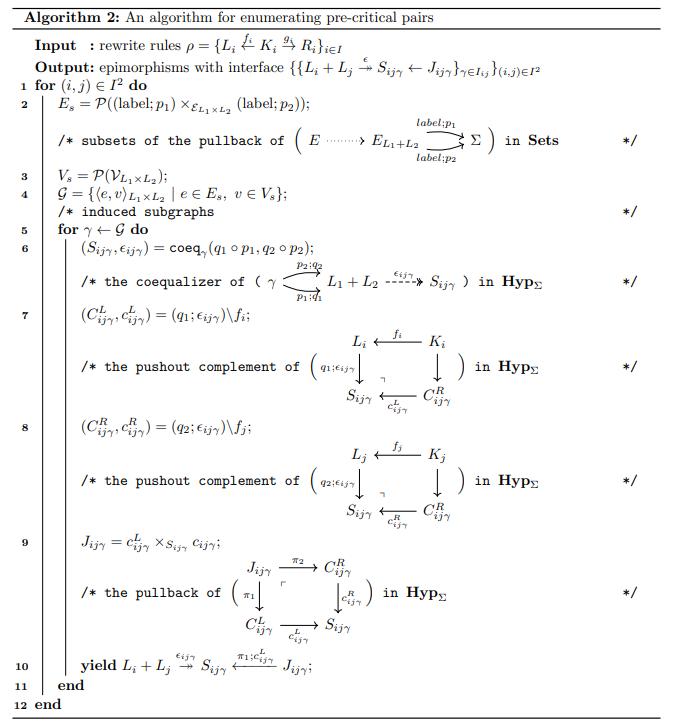
\includegraphics[scale=0.4]{images/algorithm.png} 

\end{frame}

\begin{frame}{Conjectures}
\begin{myproposition}
\begin{enumerate}
        \item \label{item:correctness} (Correctness) Each result $L_i + L_j \overset{\epsilon_{ij\gamma}}{\twoheadrightarrow} S_{ij\gamma} \xleftarrow{\pi_1;c_{ij\gamma}^L} J_{ij\gamma}$ of Algo. is a pre-critical pair.
\end{enumerate}
\end{myproposition}

\begin{myconjecture}
    \noindent
    \begin{enumerate}
        \item \label{item:exhaustiveness} (Exhaustiveness) Any pre-critical pair $L_1 + L_2 \overset{\epsilon}{\twoheadrightarrow} X \overset{F}{\leftarrow} J$ can be yielded by Algo.
    \end{enumerate}
\end{myconjecture}
\begin{myconjecture}
    Given two rewrite rules $L_i \xleftarrow{f_i} K_i \xrightarrow{g_i} R_i$ where $i \in \{1,2\}$,
    a pre-critical pair $L_1 + L_2 \overset{\epsilon}{\twoheadrightarrow} S \xleftarrow{c} J$ is parallel iff the following holds:
    \begin{enumerate}
        \item no edges from $L_1$ and $L_2$ are glued, and
        \item if two nodes from $L_1$ and $L_2$ are glued, they are in the image of $f_1$ and $f_2$.

    \end{enumerate}
\end{myconjecture}
We have proof sketches; details to be worked out.
\end{frame}

\begin{frame}{Future work}
    \begin{itemize}
        \item Optimise the algorithm.
        \item Go from SMC - with Frobenius structure - to SMC without Frobenius structure and SMCC . %for which we already have an algorithm,
        \begin{itemize}
            \item In the latter case we will need to introduce a definition for critical pairs. 
        \end{itemize}
        \item Filter out precritical pairs to return only critical pairs.
        \item (Long-shot goal:) validate compiler optimisation using critical pair analysis.
        \begin{itemize}
            \item This is shown to be possible for term rewriting \cite{DBLP:conf/flops/MuroyaH24}.
        \end{itemize}
        \item Have an Idris formalisation of our work (Juan was working on it).
    \end{itemize}
\end{frame}

\bibliographystyle{apalike}
\bibliography{ref}
\end{document}	% Done!